\section{Background}\label{sec:background}
Virtualization technique has been used in many fields, e.g.
virtual memory for resource virtualization, VMware and VirtualBox for CPU virtualization,
and Java bytecode and .Net CIL for application virtualization.
This paper discusses another application of virtulization technique
in protecting software programs from unauthorized analyses,
namely code virtualized obfuscation or VM-based obfuscation,
like VMProtect \cite{vmp} and Code Virtualizer \cite{cv}.
As software does not have uniform security requirements throughout its execution \cite{geneiatakis2012adaptive}
and protecting the whole program is too costly,
code virtualized obfuscation usually protects only the critical part(s) of the whole software program,
which could be a critical algorithm or a processing logic.
VM-based obfuscation protects a target program by transforming its native machine code into bytecode
for a self-defined virtual instruction set architecture.
At runtime, the execution instruction semantics of the original program are fulfilled
by a native interpreter bundled with the bytecode.
In this section, we will look into the internal working mechanism of VM-based obfuscation.

%\subsection{The Internals of VM-based Obfuscation}
Figure \ref{fig:vmprotection} shows the architecture of a VM-based obfuscation system.
The core of a VM-based obfuscation are the virtual IS (Instruction Set) and the native interpreter.
Virtual instructions are used to emulate native instructions.
It is required that virtual IS be able to emulate all the semantics of native IS,
or formally speaking, virtual IS should be Turing-equivalent to the native IS.
The native interpreter is to fetch and execute bytecode instructions.
It follows the \textit{decode-dispatch} approach \cite{ghosh2012replacement},
and consists of a bundle of \texttt{handlers} and a \texttt{VMloop}.
\texttt{VMloop} is the main \textit{decode-dispatch} loop and for each loop,
\texttt{VMloop} fetches a bytecode instruction, decodes it, and dispatches a \texttt{Handler} to interpret it.
Different from native instructions, bytecode instructions are specific for a virtual context,
namely \texttt{VMcontext}, which contains the virtual registers and flags.
Virtual registers and flags are related to the native registers and flags.
At runtime, \texttt{VMinit} first saves native context and uses them to initialize the virtual context.
In the simplest implementation, the virtual context could be a block of memory
and stores the exact values of the native context;
this could be more complex \cite{falliere2009inside},
but it should be guaranteed that the converting between native context and virtual context is reversible,
since \texttt{VMexit} will restore the native context from the virtual context upon exiting the virtual interpreter.


\begin{figure}[!t]
\centering
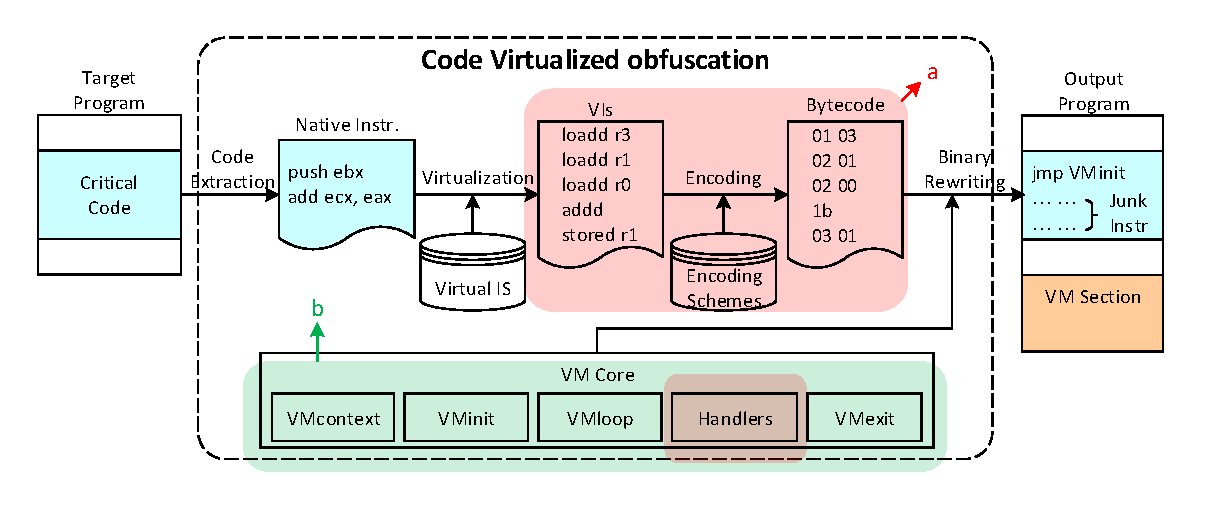
\includegraphics[width=0.9\textwidth]{fig/vmprotection.pdf}
\caption{The architecture of code virtualized obfuscation and the execution view of a VM-obfuscated program. The main work of this paper is to improve the core steps of VM-based protection (areas of ``a" and ``b"). In the ``a" region, we adopt the partition bytecode encoding schemes, and obfuscate \texttt{handlers} to generate multiple sets of \texttt{handlers}. In the ``b" region, we use a variety of methods of obfuscation and anti-taint analysis technology to protect the important components of virtual interpreter.}
\label{fig:vmprotection}
\end{figure}


Figure \ref{fig:vmprotection} also depicts the workflow of the obfuscation process. It starts from extracting the critical code from the target program. This is typically done with the help of the program author who will mark the location and scope of the critical code to be protected during programing; the obfuscation system then will search for the marks to locate the critical code at obfuscation time. The critical code is disassembled into native disassembly instructions to enable later conversion from native instructions to virtual instructions in an instruction-by-instruction fashion. The rules of conversions are set ahead of protection and are stable inside a VM-based obfuscation system. These rules depend on the semantics of the virtual IS and guarantee that the semantics of the resulted virtual instructions are equivalent to the native ones. Subsequently, virtual instructions are encoded into bytecode program. Finally, the bytecode program and other VM components are assembled into the target program through binary rewriting.
This paper improves the core steps of code virtualization protection. We modify the encoding schemes and adopt the partition bytecode programming, and generate multiple sets of \texttt{handlers}. So the bytecodes will have different semantics in different parts of bytecode program. We also use a variety of methods of obfuscation and anti-taint analysis technology to protect the critical components of virtual interpreter (section~\ref{sec:VI-Bytecode}).

At runtime, upon executing the ``critical code", an instruction, \texttt{jmp VMinit}, transfers the control to \texttt{VMinit} (Step \ding{182}). \texttt{VMinit} saves the native context and initializes the virtual context. Next, \texttt{VMloop} starts to work. It fetches a bytecode instruction, decodes it (Step \ding{183}) and dispatches a \texttt{handler} to interpret it (Step \ding{184}). Step \ding{183} and Step \ding{184} are iterated until all the bytecode instructions are interpreted. Then, \texttt{VMloop} transfers the execution to \texttt{VMexit} (Step \ding{185}), where the native context is restored and the program jumps back to the native instruction following the critical code (Step \ding{186}) and continue to execute the rest of the program code. 